\section{Differential branching fraction of the decay \btokpipimumu}

Given the statistics available for this channel, the differential branching fraction,
$\dBF(\btokpipimumu)\dqsq$ was calculated in bins of \qsq.
The differential branching fraction for a bin of width $\Delta\qsq$ is
\begin{multline}
  \frac{d}{\dqsq}\BF\left(\btokpipimumu\right)
  =
  \frac{1}{\Delta\qsq} \cdot
  \frac{\num{sig}}{\num{norm}} \cdot
  \frac{\eff{norm}}{\eff{sig}} \\
  \times\BF\left(\btokpipimumu\right) \cdot
  \BF\left(\psitwostojpsipipi\right) \cdot
  \BF\left(\jpsitomumu\right),
\end{multline}
where \num{sig} is the yield of the signal decay \btokpipimumu in the given \qsq bin and \num{norm}
is the yield of the normalization channel.
Total efficiencies for reconstruction and selection are denoted by \eff{sig} and \eff{norm} for the
signal and normalization channels respectively.

The normalization channel was chosen to be \btopsitwosk, where \psitwostojpsipipi and \jpsitomumu,
which has a total brnaching fraction of $(1.264 \pm 0.0052)\e{-5}$~\cite{PDG2012}.
This was chosen for the normlization channel over the decay \btojpsikpipi because it has a relavive
uncertainty of $4\,\%$ rather than $16\,\%$ for $\BF(\btojpsikpipi) = (8.1\pm1.3)\e{-4}$.





%Due to the high statistics of the decay \btokpipimumu, its braching fraction was also measured
%differentially, in bins of the invariant mass squared of the dimuon system (\qsq).

%Measurements pertaining to the decay \btokpipimumu were made with respect to the normalization
%channel \btopsitwosk, where \psitwostojpsipipi and \jpsitomumu.
%\begin{equation}
  %\BF\left(\b\right)
%\end{equation}





%The decay \btojpsikpipi was used for cross-checks
%These measurements were made with respect to the normalization channels




\begin{figure}
  \begin{center}
    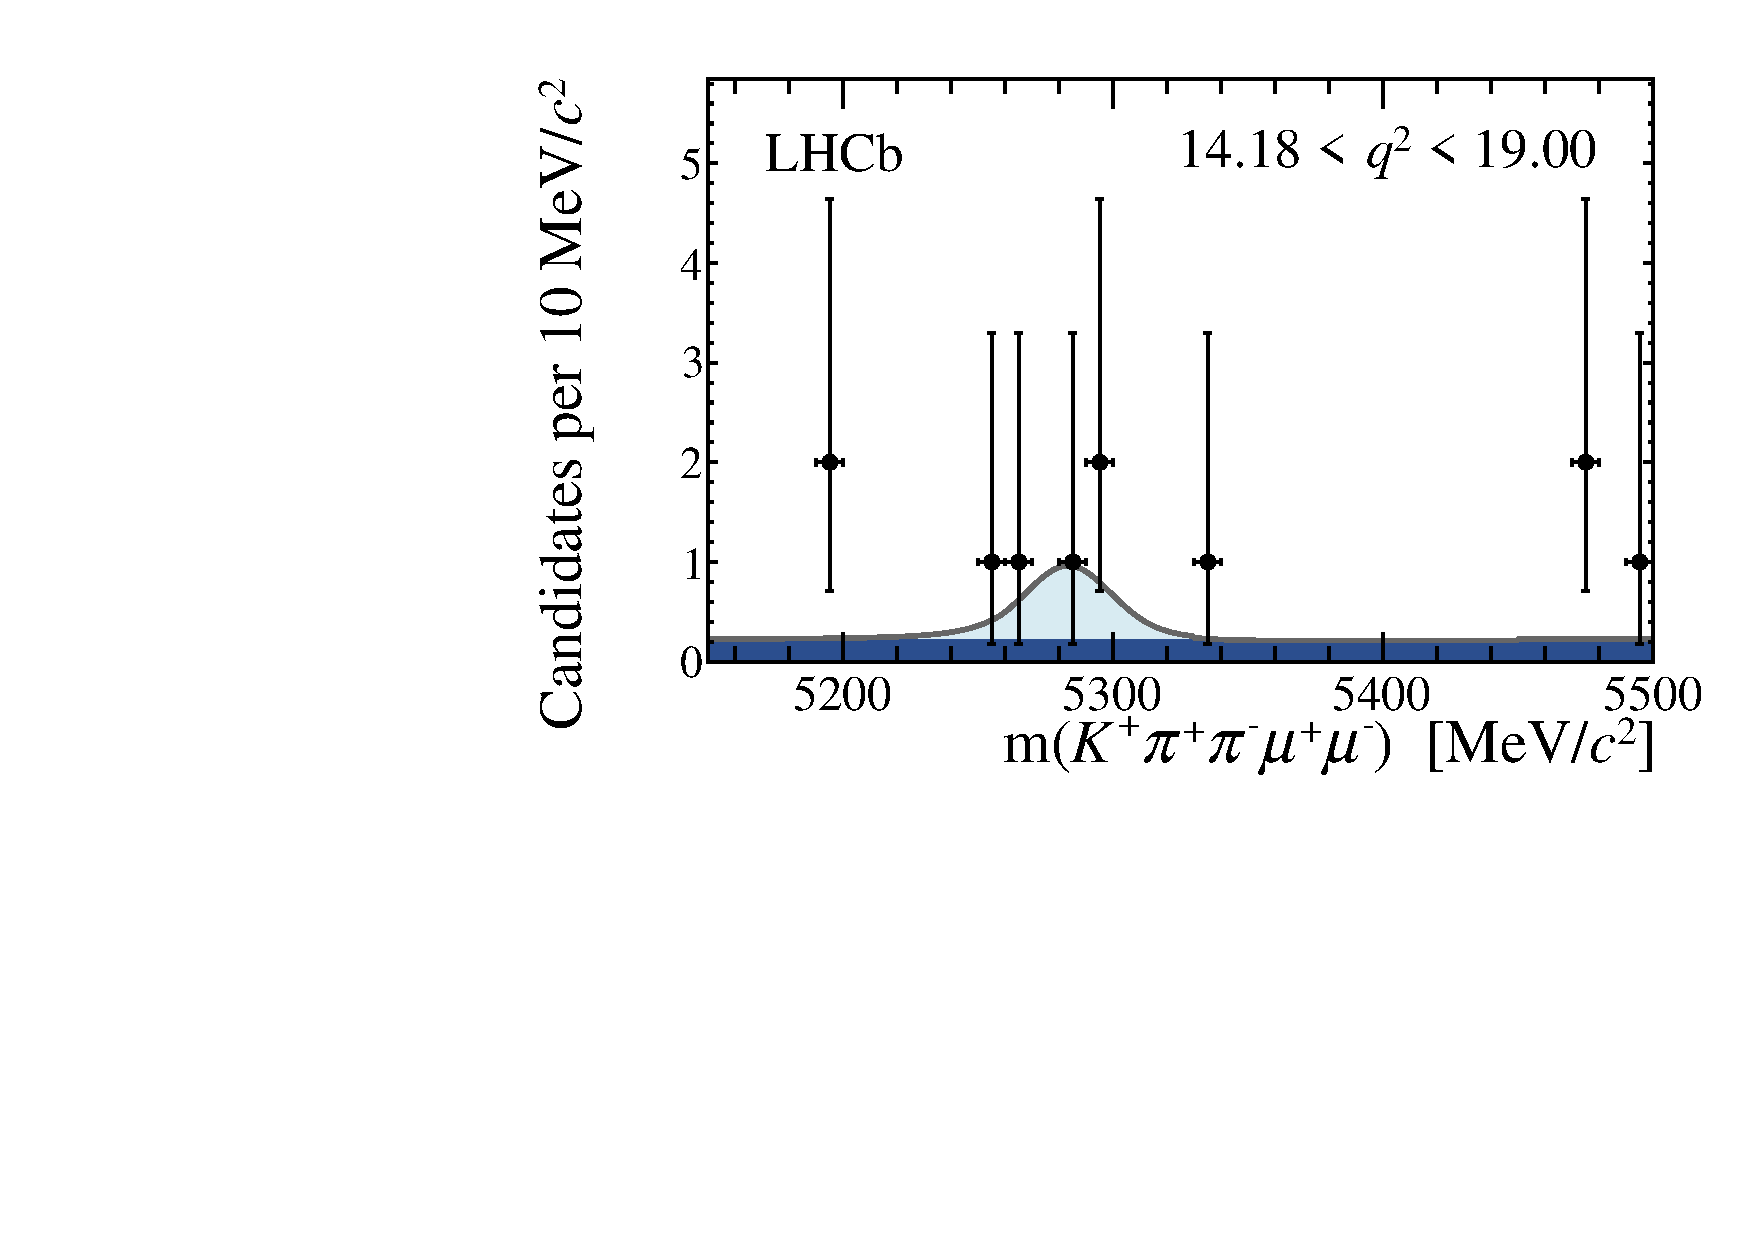
\includegraphics[width=0.48\textwidth]{q2_r6}
    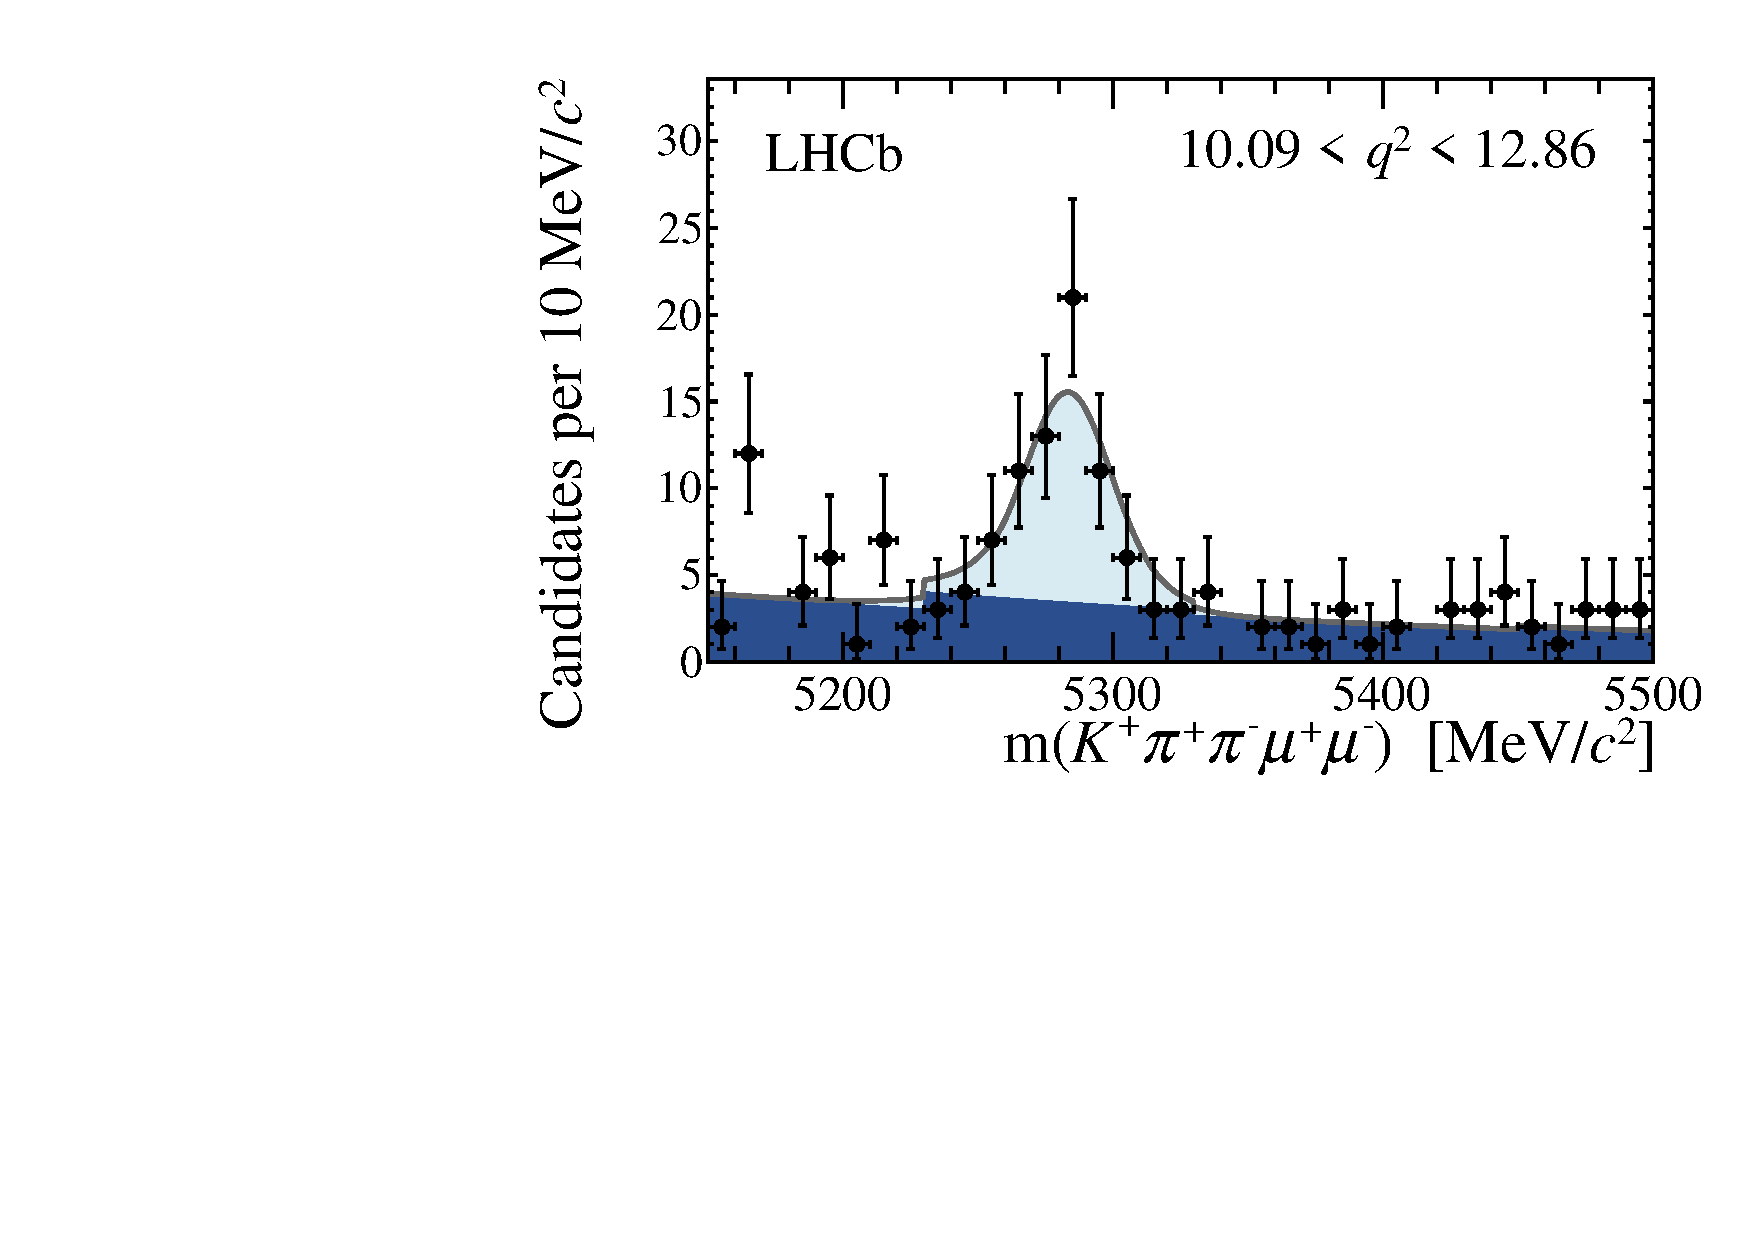
\includegraphics[width=0.48\textwidth]{q2_r5}
    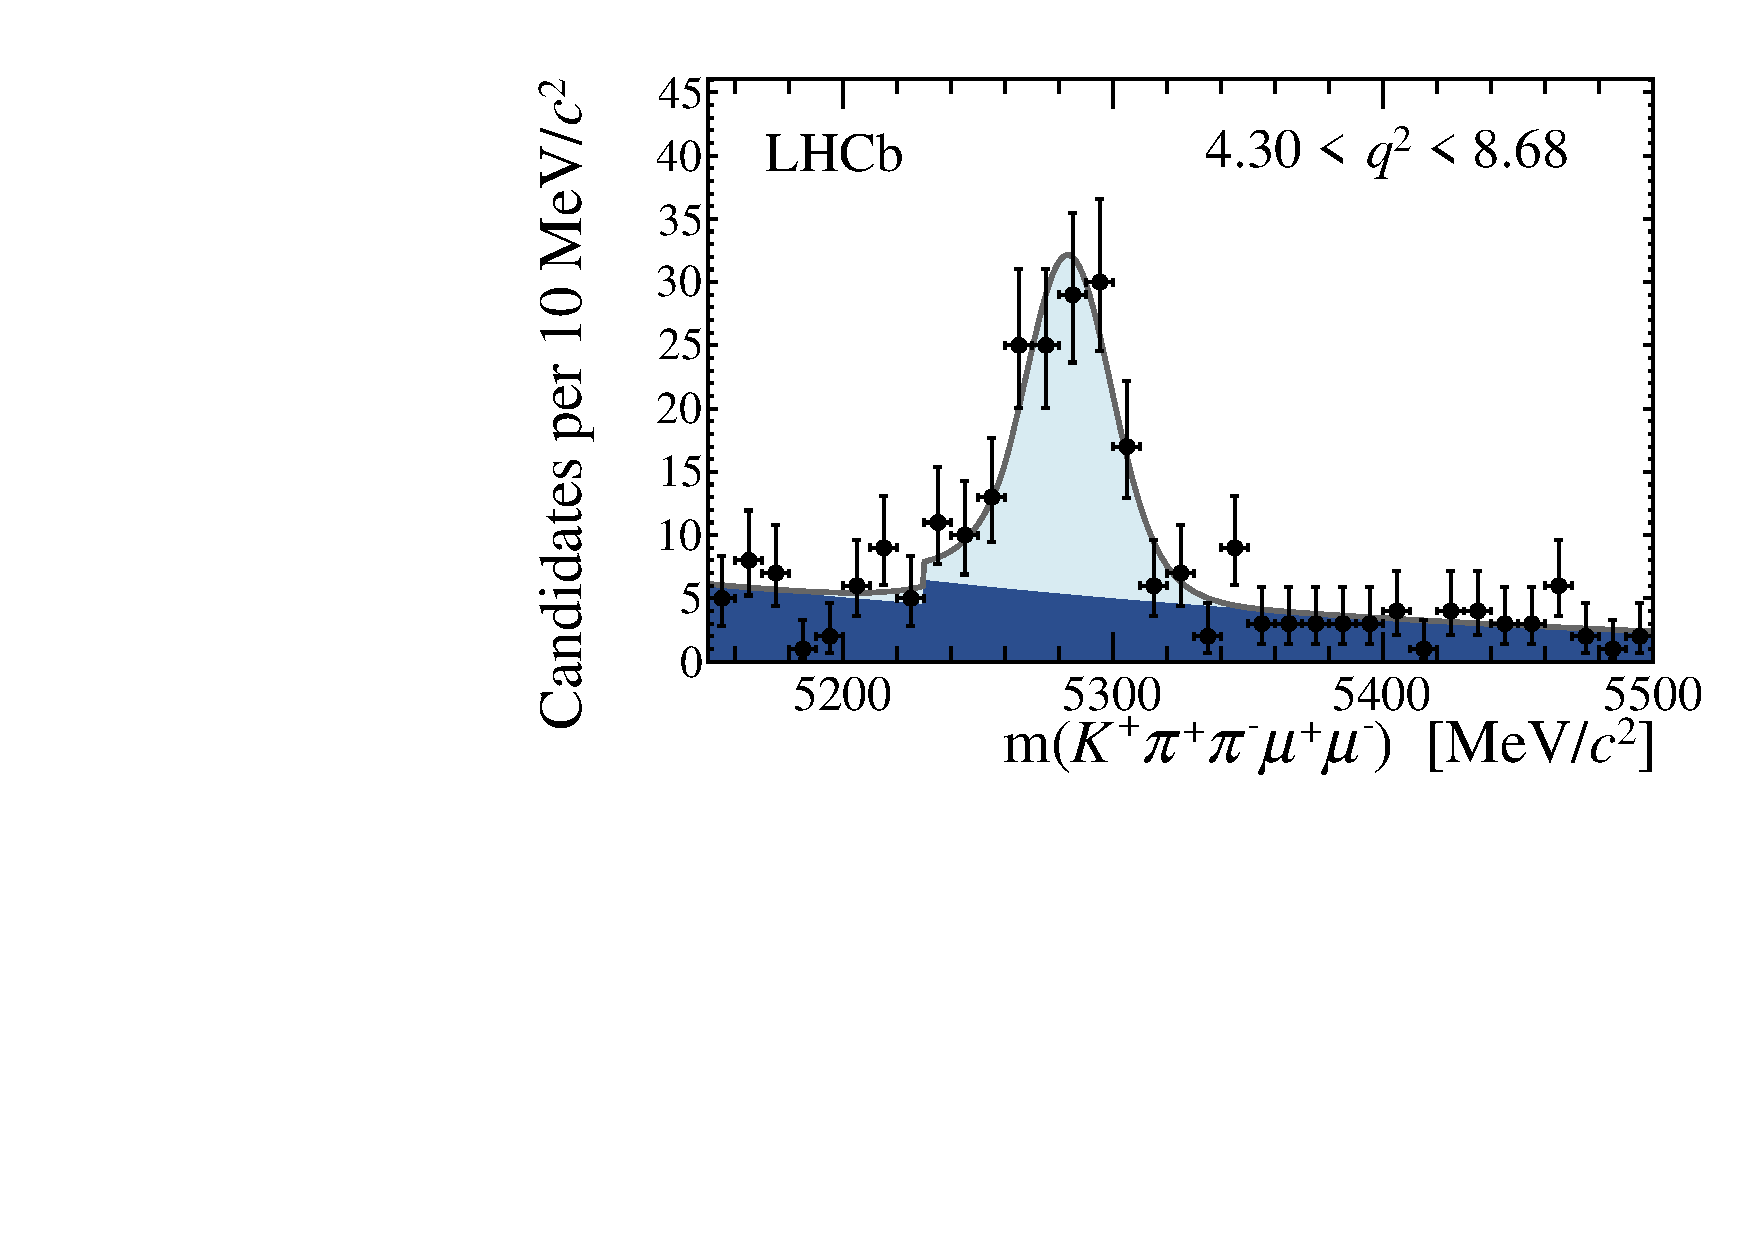
\includegraphics[width=0.48\textwidth]{q2_r4}
    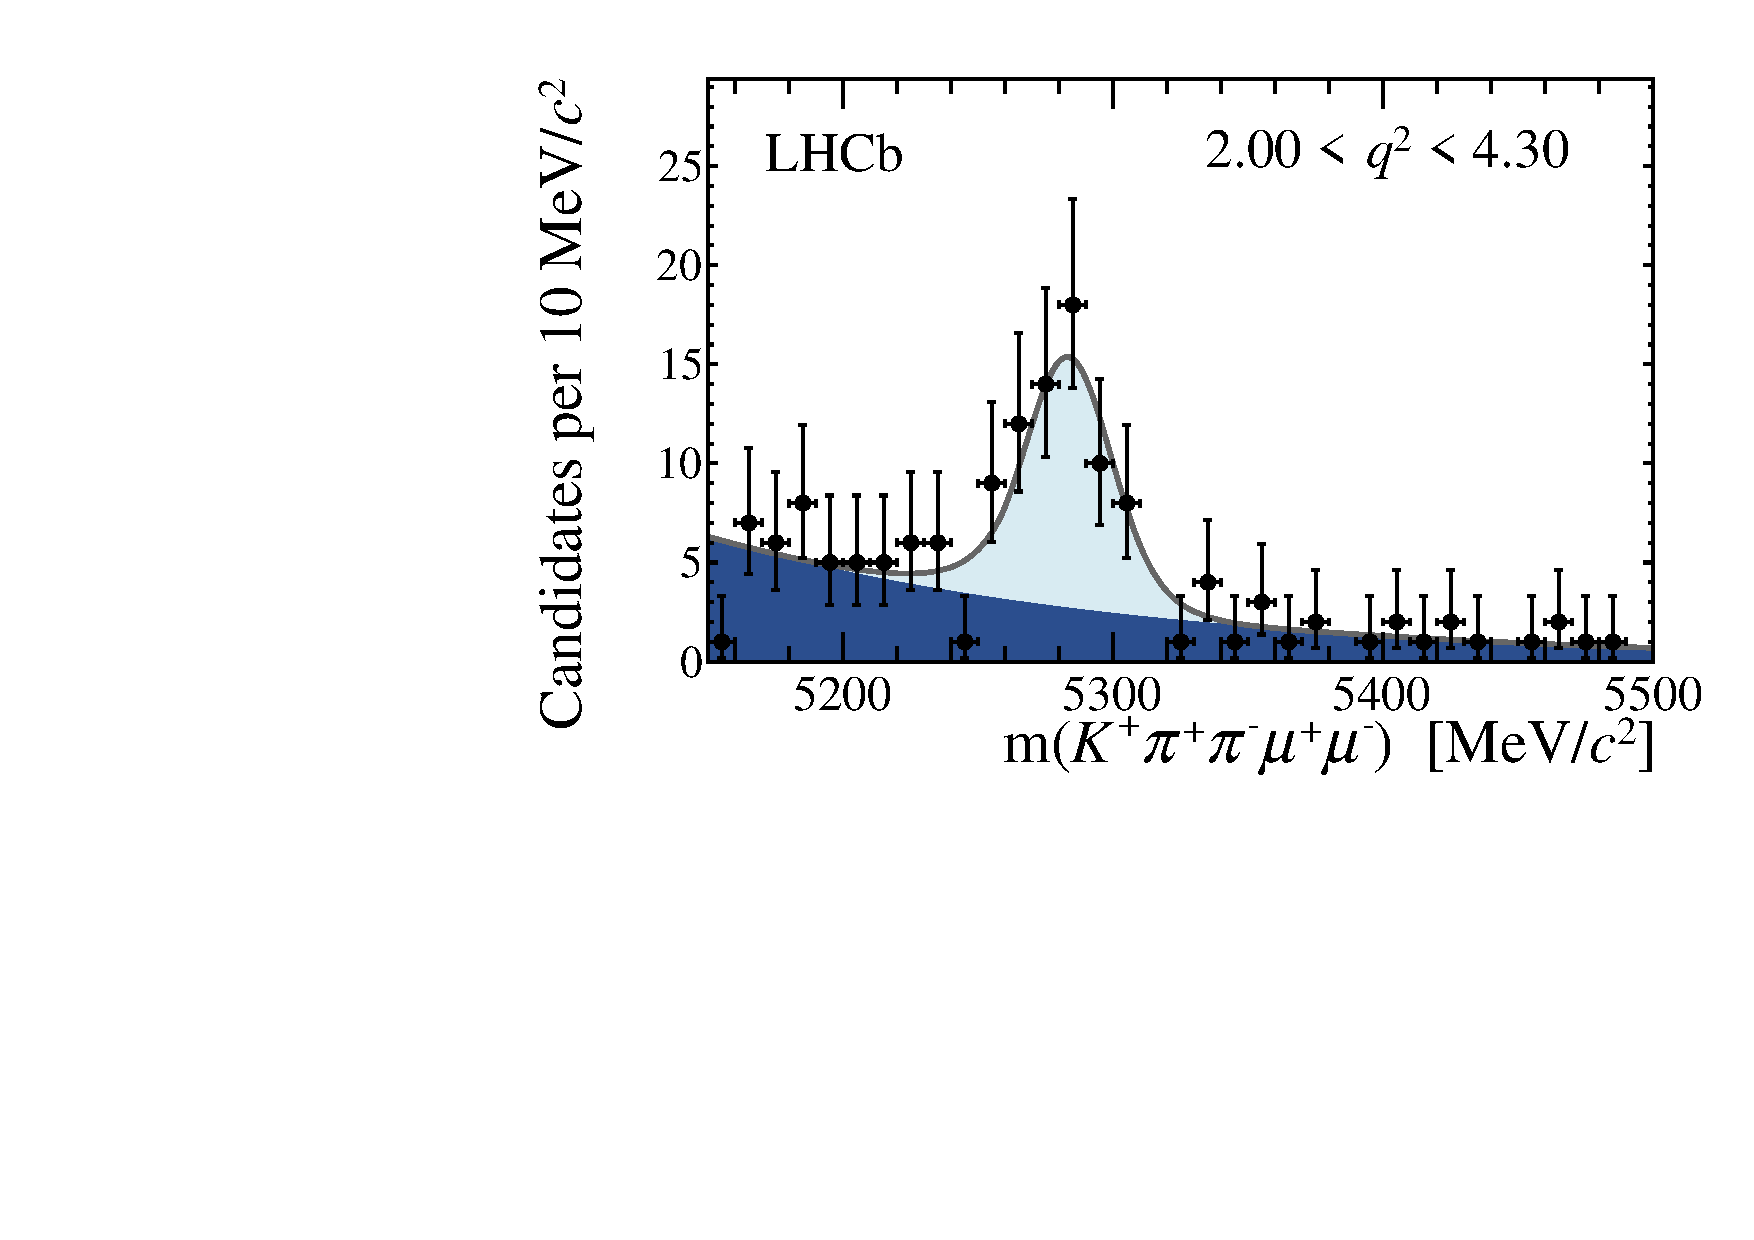
\includegraphics[width=0.48\textwidth]{q2_r3}
    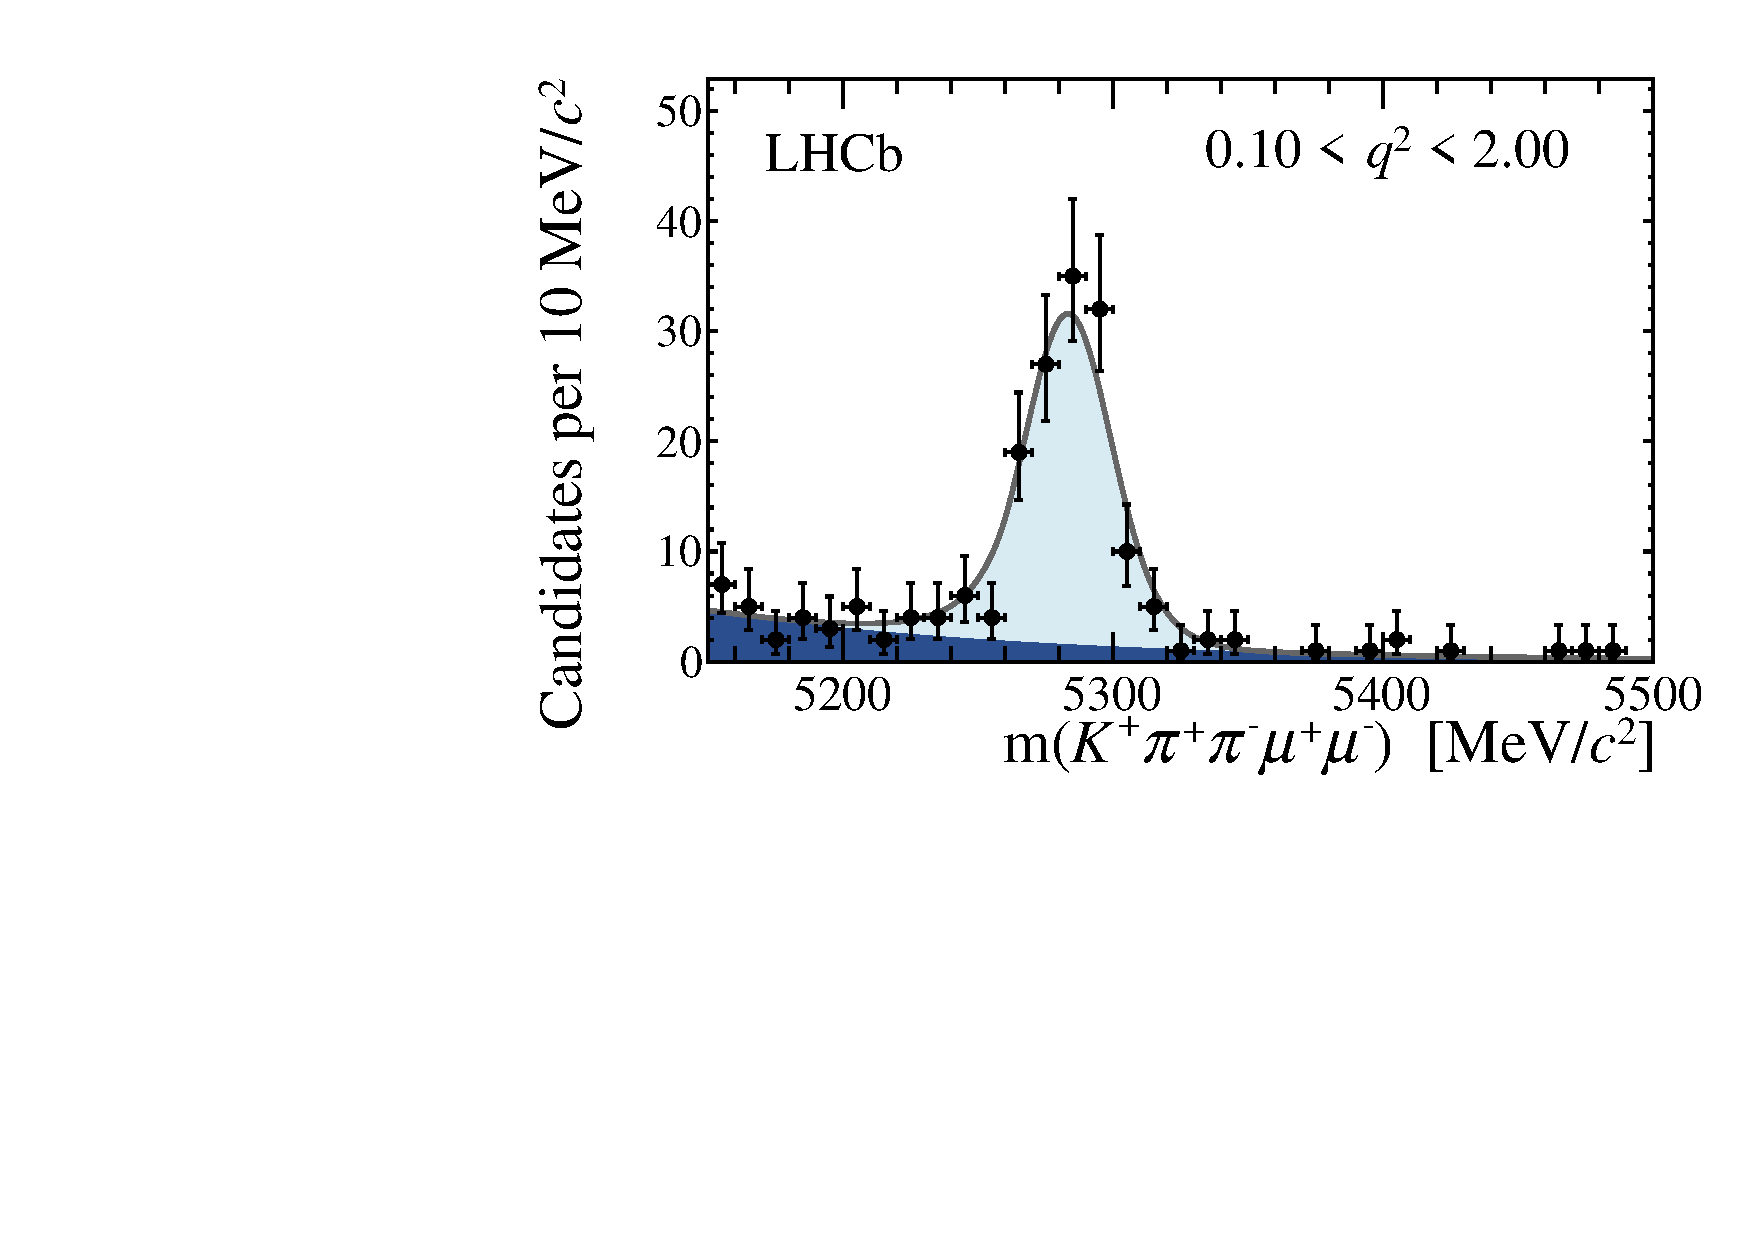
\includegraphics[width=0.48\textwidth]{q2_r2}
    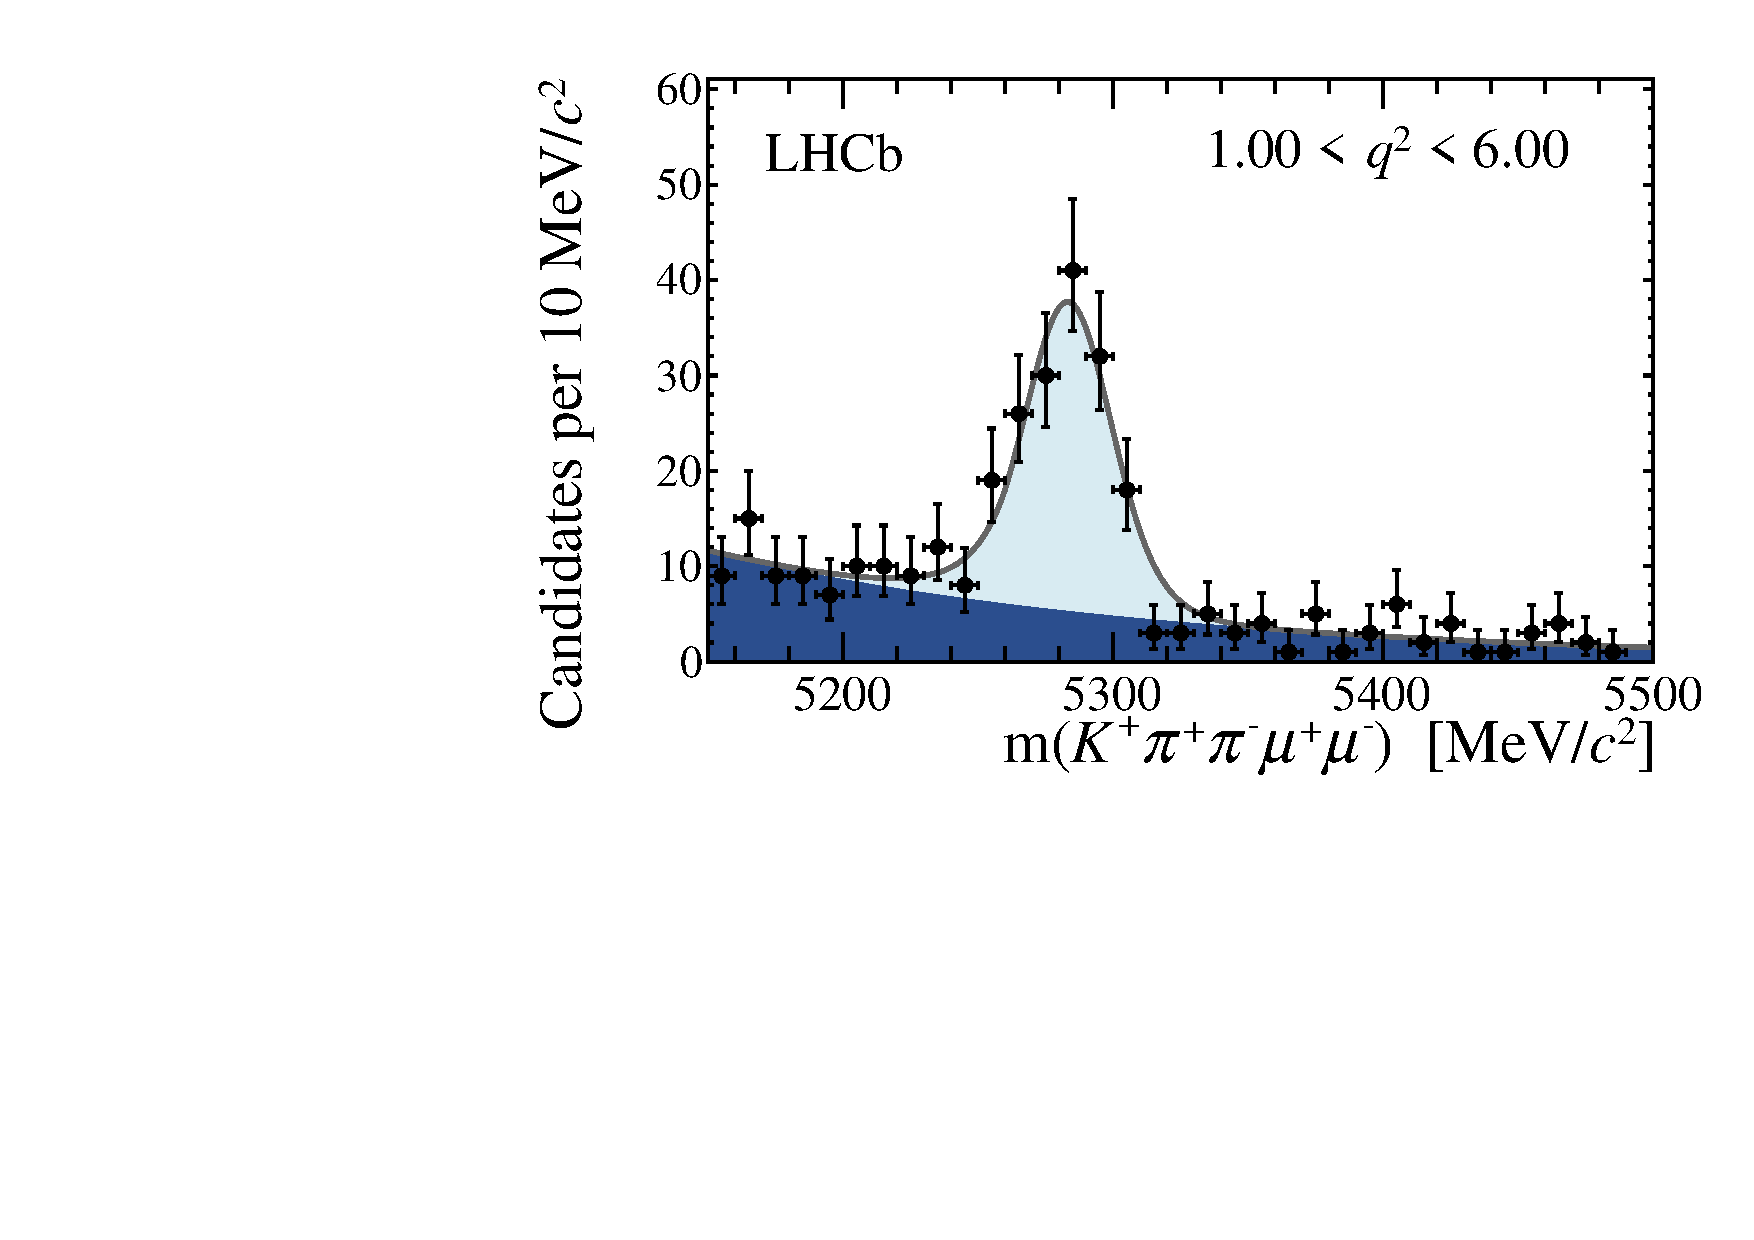
\includegraphics[width=0.48\textwidth]{q2_r1}
    \caption{\small
      Invariant mass distriburtions of \btokpipimumu candidates in bins of \qsq with projections of
      fits overlaid.
      The signal signal component (light blue) is modelled by the sum of two Gaussian
      distributions, and the background component (dark blue) is an exponential function.
      In the three \qsq bins $4.30<\qsq<8.68\gevgev$, $10.09<\qsq<12.86\gevgev$, and
      $14.18<\qsq<19.00\gevgev$ scaling factors in the background components are used to account
      the removal of the radiative tails of charmonium vetoes.
      The lower right
    }
    \label{}
  \end{center}
\end{figure}






